\documentclass[12pt,fleqn]{article}
\setlength{\parindent}{0pt}
\usepackage{graphicx}
\usepackage{listings}
\usepackage[latin5]{inputenc}
\setlength{\parskip}{8pt}
\setlength{\parsep}{0pt}
\setlength{\headsep}{0pt}
\setlength{\topskip}{0pt}
\setlength{\topmargin}{0pt}
\setlength{\topsep}{0pt}
\setlength{\partopsep}{0pt}
\setlength{\mathindent}{0cm}

\begin{document}
MIT OCW Cok Degiskenli Calculus - Ders 5

Bir cizginin formulunu iki duzlemin kesisimi olarak gorduk, fakat bu
sekilde bir tanim cogunlukla bir cizgiyi tanimlamak icin en rahat / uygun
yol degildir, cunku elinizde bazi denklemler var, bunlari cozmekle ugrasmak
lazim, vs. 

Soyle bir yontem daha iyi olmaz mi? Cizgi uzerinde bir nokta hayal edelim,
ve bu noktanin, her zaman adiminda, cizgimizin oldugu yerlerden gectigini
dusunelim. Bu tur denklemlere parametrik denklem ismi veriliyor. 

Ornek

Cizgi uzerinde iki nokta verelim. 

\[ Q_0 = (-1,2,2) \]

\[ Q_1 = (1,3,-1) \]

Guzel, bu iki nokta var ama otekilerini nasil tanimlariz? Bu iki noktatinin
arasinda, sonrasinda, oncesinde olan tum noktalar da cizgiye dahildir. 

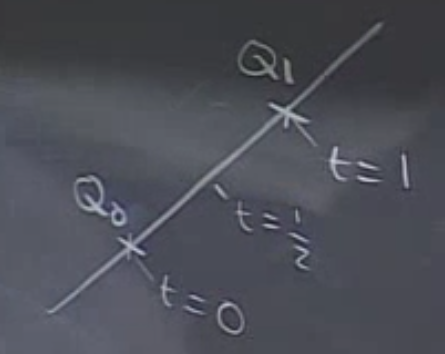
\includegraphics[height=4cm]{5_1.png}

Zaman araliklarini oyle dusunelim ki zaman indeksi sifir ($t=0$)
noktasinda, cizgi $Q_0$ uzerinde, tek birim adim atildiginda ($t=1$)  $Q_1$
uzerinde, gibi. O zaman yarim birim zamanda tam iki nokta ortasinda. 

Boylece cizgiyi temsil etmenin yolu onu $t$ bazinda hareket eden noktanin
gectigi yerler olarak tanimlamak. Bu temsilin en basit hali eger hareket
sabit hizda olursa olur. 

$t$ anindaki pozisyon $Q(t)$ nedir? 

Sorunun cevabini soyle vermeye baslayabiliriz: $\vec{Q_0Q(t)}$ vektoru
$\vec{Q_0Q_1}$ birbiriyle ortalidir. Bu oranti neye esittir? 

Bu oran $t$'ye esittir. O zaman

\[ \vec{Q_0Q(t)} = t \ \vec{Q_0Q_1}  \]

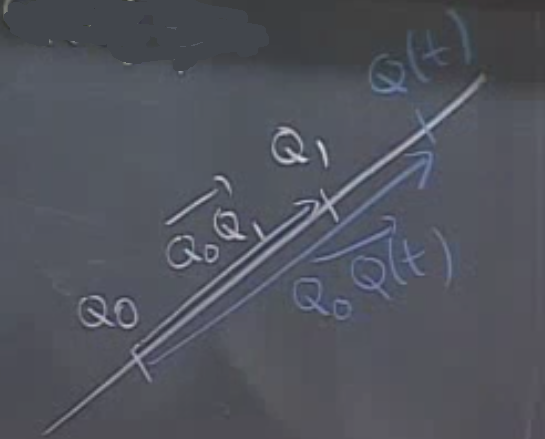
\includegraphics[height=4cm]{5_2.png}




\end{document}
